\clearpage % Rozdziały zaczynamy od nowej strony.
\section{Wyniki eksperymentów}

W niniejszym rozdziale przedstawiono wyniki przeprowadzonych eksperymentów badających możliwości autonomicznego generowania konfiguracji Infrastructure as Code przez agenty oparte na dużych modelach językowych. Analiza wyników zorganizowana jest zgodnie ze strukturą hipotez badawczych przedstawionych w rozdziale 4 — dla każdej z pięciu hipotez (H1–H5) zaprezentowano wyniki eksperymentalne, analizę danych oraz wnioski dotyczące weryfikacji hipotezy. Rozdział kończy synteza wyników podkreślająca kluczowe obserwacje dotyczące zdolności LLM do generowania IaC.

\subsection{Przegląd przeprowadzonych eksperymentów}

Eksperymenty przeprowadzono zgodnie z metodologią opisaną w rozdziale 4, wykorzystując system orkiestracji umożliwiający automatyczne wykonanie serii testów dla różnych kombinacji modeli, repozytoriów i wariantów konfiguracji. Szczegóły zbiorów danych, środowiska wykonawczego oraz metryk znajdują się w rozdziale 4.

\subsection{Wyniki H1: Autonomiczna generacja funkcjonalnych konfiguracji}

\subsubsection{Wyniki ilościowe}

\textbf{Współczynnik sukcesu ogólny:}

Łącznie 94/150 przebiegów zakończyło się sukcesem end-to-end, co daje 62{,}7\% (95\% CI: 54{,}7\%--70{,}0\%). Oznacza to, że w ponad 60\% przypadków agent był w stanie wygenerować konfigurację IaC umożliwiającą poprawne zbudowanie, wdrożenie i uruchomienie aplikacji testowej.

\textbf{Analiza etapowa i warunkowa:}

Kaskadę sukcesu między etapami pipeline'u przedstawiono na rysunku~\ref{fig:h1-funnel}. Wartości zbiorcze dla poszczególnych etapów oraz metryk warunkowych zestawiono w tabeli~\ref{tab:h1-stages}.

\begin{figure}[h]
    \centering
    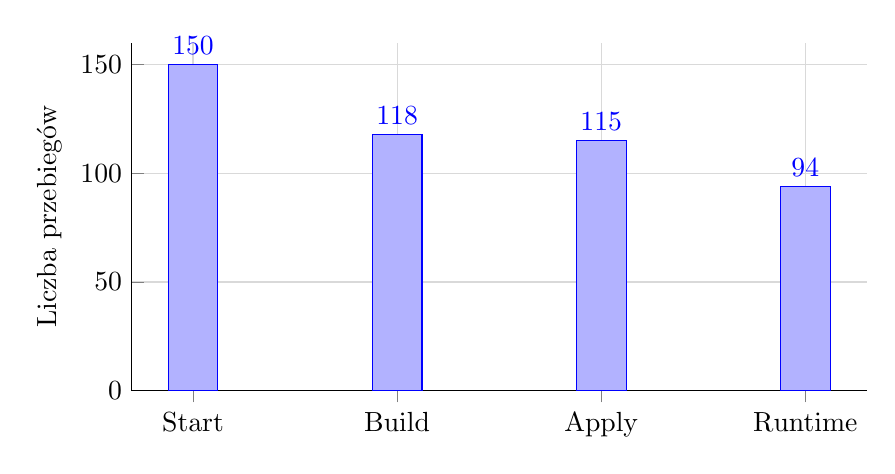
\begin{tikzpicture}
        \begin{axis}[
            ybar,
            bar width=18pt,
            ymin=0,
            ymax=160,
            width=0.9\textwidth,
            height=6cm,
            symbolic x coords={Start,Build,Apply,Runtime},
            xtick=data,
            ylabel={Liczba przebiegów},
            nodes near coords,
            nodes near coords align={vertical},
            axis x line*=bottom,
            axis y line*=left,
            grid=both,
            major grid style={draw=gray!30},
        ]
            \addplot coordinates {
                (Start,150)
                (Build,118)
                (Apply,115)
                (Runtime,94)
            };
        \end{axis}
    \end{tikzpicture}
    \caption{Kaskada sukcesu w H1: liczba przebiegów na etapach pipeline'u}
    \label{fig:h1-funnel}
\end{figure}

\begin{table}[h]
    \centering
    \begin{tabular}{lccc}
        \textbf{Etap} & \textbf{Sukcesy} & \textbf{Skuteczność} & \textbf{95\% CI} \\
        Build & 118/150 & 78{,}7\% & 71{,}4\%--84{,}5\% \\
        K8s apply & 115/148 & 77{,}7\% & 70{,}3\%--83{,}7\% \\
        apply $|$ build & 115/118 & 97{,}5\% & 92{,}8\%--99{,}1\% \\
        Runtime & 94/150 & 62{,}7\% & 54{,}7\%--70{,}0\% \\
        runtime $|$ apply & 94/115 & 81{,}7\% & 73{,}7\%--87{,}7\% \\
    \end{tabular}
    \caption{Skuteczność etapów w H1}
    \label{tab:h1-stages}
\end{table}

\textbf{Komentarz:} Największy spadek skuteczności następuje między etapem \textit{apply} a \textit{runtime}, co wskazuje, że część konfiguracji przechodzi walidację składniową i wdrożenie, ale zawodzi w uruchomieniu aplikacji. Dodatkowo, zauważalny ubytek pojawia się już na etapie budowy obrazów, co sugeruje, że problemy zależności i kontekstu budowania są istotnym źródłem błędów.

\textbf{Rozbicie per model:}

Porównanie skuteczności modeli znajduje się w tabeli~\ref{tab:h1-models}.

\begin{table}[h]
    \centering
    \begin{tabular}{lccc}
        \textbf{Model} & \textbf{Sukcesy} & \textbf{Skuteczność} & \textbf{95\% CI} \\
        gemini-2.5-flash & 31/50 & 62{,}0\% & 48{,}2\%--74{,}1\% \\
        gpt-5-mini & 34/50 & 68{,}0\% & 54{,}2\%--79{,}2\% \\
        deepseek-chat & 29/50 & 58{,}0\% & 44{,}2\%--70{,}6\% \\
    \end{tabular}
    \caption{Skuteczność per model w H1}
    \label{tab:h1-models}
\end{table}

\textbf{Rozbicie per repozytorium:}

Rozkład skuteczności dla poszczególnych projektów pokazuje tabela~\ref{tab:h1-repos}.

\begin{table}[h]
    \centering
    \begin{tabular}{lccc}
        \textbf{Repozytorium} & \textbf{Sukcesy} & \textbf{Skuteczność} & \textbf{95\% CI} \\
        math-pdf-generator-web & 6/6 & 100{,}0\% & 61{,}0\%--100{,}0\% \\
        simple-webapp & 0/6 & 0{,}0\% & 0{,}0\%--39{,}0\% \\
        banner-designer-webapp & 5/6 & 83{,}3\% & 43{,}6\%--97{,}0\% \\
        lsfont & 5/6 & 83{,}3\% & 43{,}6\%--97{,}0\% \\
        airwatch & 0/6 & 0{,}0\% & 0{,}0\%--39{,}0\% \\
        diceopt\_kcd2 & 6/6 & 100{,}0\% & 61{,}0\%--100{,}0\% \\
        parklandschooltimer & 6/6 & 100{,}0\% & 61{,}0\%--100{,}0\% \\
        realtime-chatting-webapp & 1/6 & 16{,}7\% & 3{,}0\%--56{,}4\% \\
        csv-hero & 2/6 & 33{,}3\% & 9{,}7\%--70{,}0\% \\
        metathief & 3/6 & 50{,}0\% & 18{,}8\%--81{,}2\% \\
        deeplx-app & 6/6 & 100{,}0\% & 61{,}0\%--100{,}0\% \\
        mtg-scryfall-randomizer & 6/6 & 100{,}0\% & 61{,}0\%--100{,}0\% \\
        vesen & 3/6 & 50{,}0\% & 18{,}8\%--81{,}2\% \\
        webclient & 2/6 & 33{,}3\% & 9{,}7\%--70{,}0\% \\
        chessable & 4/6 & 66{,}7\% & 30{,}0\%--90{,}3\% \\
        class-order-checker & 6/6 & 100{,}0\% & 61{,}0\%--100{,}0\% \\
        adsensedetective & 1/6 & 16{,}7\% & 3{,}0\%--56{,}4\% \\
        mario-kart-tournament & 1/6 & 16{,}7\% & 3{,}0\%--56{,}4\% \\
        tempo-sync & 5/6 & 83{,}3\% & 43{,}6\%--97{,}0\% \\
        attendence-calculator & 6/6 & 100{,}0\% & 61{,}0\%--100{,}0\% \\
        scheme-seva & 2/6 & 33{,}3\% & 9{,}7\%--70{,}0\% \\
        hello-world-war & 4/6 & 66{,}7\% & 30{,}0\%--90{,}3\% \\
        openai-hello-world & 2/6 & 33{,}3\% & 9{,}7\%--70{,}0\% \\
        todo-list & 6/6 & 100{,}0\% & 61{,}0\%--100{,}0\% \\
        simple-webapp-flask & 6/6 & 100{,}0\% & 61{,}0\%--100{,}0\% \\
    \end{tabular}
    \caption{Skuteczność per repozytorium w H1}
    \label{tab:h1-repos}
\end{table}

\subsubsection{Typowe problemy i przyczyny awarii}

Poniżej zebrano najczęstsze przyczyny niepowodzeń obserwowane w H1:

\begin{itemize}
    \item \textbf{Problemy z zależnościami NPM:} agent używa \texttt{npm ci} lub \texttt{npm ci --omit=dev}, co zawodzi przy braku \texttt{package-lock.json} lub gdy zależności są błędnie oznaczone jako dev (np. brak \texttt{vite} w runtime).
    \item \textbf{Błędne kopiowanie plików:} próba kopiowania \texttt{package-lock.json}, gdy nie istnieje, oraz kopiowanie z niepoprawnego kontekstu budowania (np. \texttt{COPY back-end/ ./} przy braku katalogu).
    \item \textbf{Konflikt użytkownika w kontenerze:} błąd \texttt{runAsNonRoot} w Kubernetes przy obrazie uruchamianym jako root.
    \item \textbf{Read-only filesystem w runtime:} aplikacje oparte o Nginx nie mogą utworzyć katalogów roboczych (np. \texttt{/var/cache/nginx/client\_temp}).
    \item \textbf{Nieprawidłowe \texttt{imagePullPolicy}:} ustawienie \texttt{Never} uniemożliwia pobranie obrazu.
    \item \textbf{Nieaktualne obrazy bazowe:} zbyt stary base image powoduje błędy \texttt{apt} podczas budowy.
    \item \textbf{Niezgodne wersje środowiska:} agent nie rozpoznaje konfliktów wersji (np. Node 18 w base image nie wspiera zależności aplikacji), brakuje mu wiarygodnego źródła informacji o takich ograniczeniach.
    \item \textbf{Błędny \texttt{test\_endpoint}:} agent wybiera niepoprawny endpoint zdrowia mimo działającej aplikacji pod \texttt{/}.
    \item \textbf{Błędy importu w Pythonie:} uruchamianie modułów z relatywnymi importami bez pakietu (np. \texttt{ImportError: attempted relative import with no known parent package}).
\end{itemize}

\textbf{Wniosek:} Dominujące błędy dotyczą środowiska uruchomieniowego i procesu budowy (wersje bazowych obrazów, kontekst kopiowania, zależności), a nie samych manifestów Kubernetes. Oznacza to, że ograniczenia H1 w dużej mierze wynikają z niedoskonałego rozpoznania środowiska aplikacji, a nie z błędów składniowych IaC.

\subsubsection{Werdykt dla H1}

Na podstawie kryteriów z rozdziału 4 hipoteza H1 została potwierdzona. Spełnienie warunków przedstawia się następująco:
\begin{itemize}
    \item end-to-end success rate: 62{,}7\% (próg 60\%),
    \item skuteczność etapów: build 78{,}7\% (próg 75\%), apply 77{,}7\% (próg 75\%), runtime 62{,}7\% (próg 60\%),
    \item metryki warunkowe: apply $|$ build 97{,}5\% (próg 95\%), runtime $|$ apply 81{,}7\% (próg 80\%),
    \item repozytoria z sukcesem $\geq$ 50\%: 16 z 25 (wymagane $\geq$ 50\% zbioru).
\end{itemize}
W konsekwencji można uznać, że agenty LLM są w stanie autonomicznie generować funkcjonalne konfiguracje IaC w badanym zakresie.

\subsection{Wyniki H2: Ograniczenia złożonościowe}

\subsubsection{Wyniki ilościowe}

\textbf{Wynik ogólny:}

Łącznie 15/45 przebiegów zakończyło się sukcesem end-to-end, co daje 33{,}3\% (95\% CI: 21{,}4\%--47{,}9\%).

\textbf{Analiza etapowa i warunkowa:}

Zestawienie skuteczności etapów oraz metryk warunkowych znajduje się w tabeli~\ref{tab:h2-stages}.

\begin{table}[h]
    \centering
    \begin{tabular}{lccc}
        \textbf{Etap} & \textbf{Sukcesy} & \textbf{Skuteczność} & \textbf{95\% CI} \\
        Build & 32/45 & 71{,}1\% & 56{,}6\%--82{,}3\% \\
        K8s apply & 24/42 & 57{,}1\% & 42{,}2\%--70{,}9\% \\
        apply $|$ build & 24/32 & 75{,}0\% & 57{,}9\%--86{,}7\% \\
        Runtime & 15/45 & 33{,}3\% & 21{,}4\%--47{,}9\% \\
        runtime $|$ apply & 15/24 & 62{,}5\% & 42{,}7\%--78{,}8\% \\
    \end{tabular}
    \caption{Skuteczność etapów w H2}
    \label{tab:h2-stages}
\end{table}

\textbf{Rozbicie per model:}

Wyniki dla poszczególnych modeli przedstawiono w tabeli~\ref{tab:h2-models}.

\begin{table}[h]
    \centering
    \begin{tabular}{lccc}
        \textbf{Model} & \textbf{Sukcesy} & \textbf{Skuteczność} & \textbf{95\% CI} \\
        gemini-2.5-flash & 3/15 & 20{,}0\% & 7{,}0\%--45{,}2\% \\
        gpt-5-mini & 7/15 & 46{,}7\% & 24{,}8\%--69{,}9\% \\
        deepseek-chat & 5/15 & 33{,}3\% & 15{,}2\%--58{,}3\% \\
    \end{tabular}
    \caption{Skuteczność per model w H2}
    \label{tab:h2-models}
\end{table}

\textbf{Rozbicie per repozytorium:}

Wyniki dla repozytoriów POC1--POC5 zestawiono w tabeli~\ref{tab:h2-repos}.

\begin{table}[h]
    \centering
    \begin{tabular}{lccc}
        \textbf{Repozytorium} & \textbf{Sukcesy} & \textbf{Skuteczność} & \textbf{95\% CI} \\
        poc1-fastapi & 9/9 & 100{,}0\% & 70{,}1\%--100{,}0\% \\
        poc2-fastapi & 3/9 & 33{,}3\% & 12{,}1\%--64{,}6\% \\
        poc3-fastapi & 2/9 & 22{,}2\% & 6{,}3\%--54{,}7\% \\
        poc4-fastapi & 1/9 & 11{,}1\% & 2{,}0\%--43{,}5\% \\
        poc5 & 0/9 & 0{,}0\% & 0{,}0\%--29{,}9\% \\
    \end{tabular}
    \caption{Skuteczność per repozytorium w H2}
    \label{tab:h2-repos}
\end{table}

Zestawienie skuteczności etapów per repozytorium znajduje się w tabeli~\ref{tab:h2-repo-stages}.

\begin{table}[h]
    \centering
    \begin{tabular}{lccc}
        \textbf{Repozytorium} & \textbf{Build} & \textbf{Apply} & \textbf{Runtime} \\
        poc1-fastapi & 9/9 (100{,}0\%) & 9/9 (100{,}0\%) & 9/9 (100{,}0\%) \\
        poc2-fastapi & 9/9 (100{,}0\%) & 7/9 (77{,}8\%) & 3/9 (33{,}3\%) \\
        poc3-fastapi & 6/9 (66{,}7\%) & 3/9 (33{,}3\%) & 2/9 (22{,}2\%) \\
        poc4-fastapi & 6/9 (66{,}7\%) & 4/7 (57{,}1\%) & 1/9 (11{,}1\%) \\
        poc5 & 2/9 (22{,}2\%) & 1/8 (12{,}5\%) & 0/9 (0{,}0\%) \\
    \end{tabular}
    \caption{Skuteczność etapów per repozytorium w H2}
    \label{tab:h2-repo-stages}
\end{table}

Wraz ze wzrostem złożoności widać silny spadek skuteczności: od 100{,}0\% dla POC1 do 0{,}0\% dla POC5, co ilustruje wykres na rysunku~\ref{fig:h2-success-vs-complexity}.

\begin{figure}[h]
    \centering
    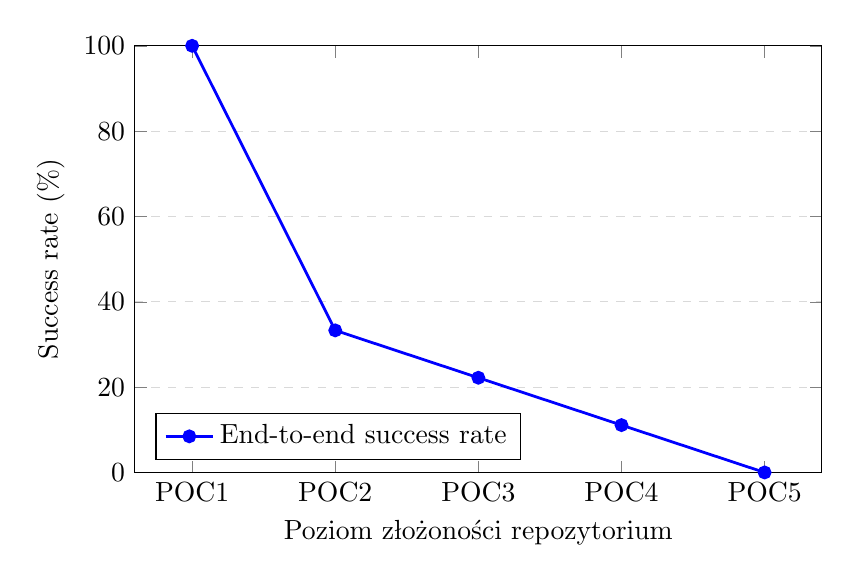
\begin{tikzpicture}
        \begin{axis}[
            width=0.85\textwidth,
            height=7cm,
            ymin=0,
            ymax=100,
            xtick={1,2,3,4,5},
            xticklabels={POC1,POC2,POC3,POC4,POC5},
            ylabel={Success rate (\%)},
            xlabel={Poziom złożoności repozytorium},
            ymajorgrids=true,
            grid style={dashed,gray!30},
            legend pos=south west,
        ]
            \addplot[
                color=blue,
                mark=*,
                line width=1pt
            ] coordinates {
                (1,100.0)
                (2,33.3)
                (3,22.2)
                (4,11.1)
                (5,0.0)
            };
            \addlegendentry{End-to-end success rate}
        \end{axis}
    \end{tikzpicture}
    \caption{Success rate a poziom złożoności (repozytoria kontrolowane)}
    \label{fig:h2-success-vs-complexity}
\end{figure}

\subsubsection{Trend złożoności}

Dane wskazują na niemal idealny trend spadkowy skuteczności wraz ze wzrostem złożoności (korelacja Spearmana $\rho \approx -1{,}0$ dla POC1--POC5). Największy spadek widoczny jest między POC1 i POC2, a kolejne poziomy złożoności przynoszą dalsze obniżenie skuteczności aż do 0\% dla POC5. Wskazuje to na punkt załamania po przekroczeniu prostej architektury wielowarstwowej, gdy dochodzą dodatkowe zależności infrastrukturalne i wzajemne powiązania usług.

\subsubsection{Typowe problemy i przyczyny awarii}

\begin{itemize}
    \item Błędna składnia sekretów w Kubernetes: niepoprawnie zakodowane pola \texttt{data} (np. \texttt{illegal base64 data}) zamiast poprawnego Base64 lub użycia \texttt{stringData}.
    \item Niepoprawne polecenie \texttt{COPY} w Dockerfile (np. brak ścieżki docelowej), co kończy się błędem \texttt{At least two arguments are required for COPY}.
    \item Uruchomienie \texttt{npm ci} bez pliku \texttt{package-lock.json} (lub bez skopiowania lockfile do obrazu), co blokuje instalację zależności.
    \item Brak nazw portów w \texttt{Service} z wieloma portami, co powoduje walidację \texttt{spec.ports[*].name: Required value}.
    \item Niezgodna wersja Pythona z adnotacjami typów (np. \texttt{models.User | None} w Pythonie < 3.10), skutkująca \texttt{TypeError}.
    \item Błędne umieszczenie dyrektywy \texttt{server} w \texttt{nginx.conf} (poza blokiem \texttt{http}), co kończy się \texttt{directive is not allowed here}.
    \item Brak usługi/bazy w Kubernetes (np. brak \texttt{Service} o nazwie \texttt{notes-db}) lub brak zmiennej środowiskowej z adresem DB, skutkujące \texttt{could not translate host name}.
    \item Błędne przekazanie zmiennych środowiskowych do bazy (np. literalne \texttt{"\$(POSTGRES\_USER)"}), co daje \texttt{password authentication failed}.
\end{itemize}

\textbf{Wniosek:} Wraz z rosnącą liczbą usług i zależności infrastrukturalnych spada nie tylko skuteczność końcowa, ale też stabilność wcześniejszych etapów. W prostych repozytoriach (POC1) pipeline przechodzi bez zakłóceń, natomiast w POC3--POC5 rośnie odsetek awarii już na etapie budowy i aplikowania manifestów, a w POC5 brak jest sukcesów runtime. Wskazuje to, że główna bariera leży w koordynacji wielu usług, ich zależności oraz poprawnym zestawieniu konfiguracji środowiskowej. Dominujące źródła porażek to błędy walidacyjne manifestów oraz problemy ze spójnością konfiguracji środowiskowej (sekrety, nazwy usług, zmienne), co potwierdza krytyczność etapu integracji.

\subsubsection{Werdykt dla H2}

Na podstawie wyników dla POC1--POC5 hipoteza H2 została potwierdzona: spełniony jest warunek trendu spadkowego ($\rho \leq -0{,}6$), a różnica skuteczności POC1--POC5 wynosi 100{,}0 p.p.

\subsection{Wyniki H3: Jakość i zgodność z dobrymi praktykami}

\subsubsection{Wyniki ilościowe}

Poniżej zestawiono wyniki jakości dla 150 przebiegów (25 repozytoriów $\times$ 3 modele $\times$ 2 warianty prompta), a szczegółowe wartości ujęto w tabeli~\ref{tab:h3-lint-summary}.

\begin{table}[h]
    \centering
    \begin{tabular}{lcccc}
        \textbf{Wariant prompta} & \textbf{Z ostrzeżeniami} & \textbf{Bez ostrzeżeń} & \textbf{Łącznie} & \textbf{Średnio} \\
        Bazowy & 62/75 (82{,}7\%) & 13/75 (17{,}3\%) & 147 (17D, 130K) & 1{,}96 \\
        Best practices & 19/75 (25{,}3\%) & 56/75 (74{,}7\%) & 30 (8D, 22K) & 0{,}40 \\
    \end{tabular}
    \caption{Ostrzeżenia Hadolint i Kube-linter w H3 (D: Dockerfile, K: Kubernetes)}
    \label{tab:h3-lint-summary}
\end{table}

\subsubsection{Wpływ prompt engineeringu}

Wzmocnienie prompta o checklistę dobrych praktyk znacząco poprawia jakość konfiguracji: łączna liczba ostrzeżeń spadła z 147 do 30 (o 79{,}6\%), a średnia liczba ostrzeżeń na przebieg z 1{,}96 do 0{,}40. Odsetek przebiegów bez ostrzeżeń wzrósł o 57{,}4 p.p. (z 17{,}3\% do 74{,}7\%), a odsetek przebiegów z ostrzeżeniami spadł z 82{,}7\% do 25{,}3\%. W obu wariantach dominowały ostrzeżenia Kube-linter, jednak spadły one z 130 do 22, co wskazuje na skuteczność wytycznych dotyczących manifestów Kubernetes.

\subsubsection{Werdykt dla H3}

Hipoteza H3 została potwierdzona. W wariancie bazowym odsetek przebiegów z ostrzeżeniami przekracza 60\% (82{,}7\%). Wariant best practices obniża łączną liczbę ostrzeżeń o 79{,}6\% oraz zwiększa odsetek konfiguracji bez ostrzeżeń o 57{,}4 p.p., co przekracza przyjęte progi weryfikacji. Wynik ten sugeruje, że nawet przy bardzo dużym kontekście wejściowym (rzędu $10^5$ tokenów na przebieg) model nadal w sposób konsekwentny respektuje dostarczone wytyczne jakościowe.

\subsection{Wyniki H4: Niezawodność i powtarzalność procesu agentowego}

\subsubsection{Wyniki ilościowe}

% TODO: run-to-run diff ratio + zmienność liczby kroków narzędziowych.

\subsubsection{Analiza powtarzalności}

% TODO: Wpływ deterministycznych parametrów (temperature=0, seed).

\subsubsection{Werdykt dla H4}

% TODO: Wniosek z odniesieniem do progów z rozdziału 4.

\subsection{Wyniki H5: Podatność na manipulację kontekstem}

\subsubsection{Wyniki ilościowe}

% TODO: Odsetek przebiegów z odchyleniami od oczekiwań.

\subsubsection{Przykłady manipulacji}

% TODO: Krótkie studia przypadków (prompt injection, myląca dokumentacja).

\subsubsection{Werdykt dla H5}

% TODO: Wniosek z odniesieniem do progów z rozdziału 4.

\subsection{Porównanie modeli}

% TODO: Analiza przekrojowa modeli (skuteczność, jakość, powtarzalność).

\subsection{Synteza wyników}

\subsubsection{Podsumowanie weryfikacji hipotez}

% TODO: Tabela zbiorcza z werdyktem dla H1–H5 i krótkim uzasadnieniem.

\subsubsection{Kluczowe wnioski}

% TODO: 3–6 punktów najważniejszych obserwacji.

\subsubsection{Ograniczenia badania}

% TODO: Wypunktuj ograniczenia wyników (zbieżne z threats to validity).

\subsubsection{Implikacje praktyczne}

% TODO: Zalecenia dla praktyków i twórców narzędzi DevOps.
